\documentclass[12pt,a4paper]{article}
\usepackage{amsmath, bm, empheq, graphicx, hyperref, multirow, physics, siunitx}
\usepackage[column=O]{cellspace}
\usepackage[extrafootnotefeatures]{xepersian}
\settextfont{XB Zar}
\title{سرمایش زیر یک کلوین}
\author{صالح شاملو احمدی\\دانشگاه صنعتی شریف، دانشکده فیزیک}

\hypersetup{colorlinks=true, citecolor=cyan, urlcolor=blue}
\setlength\cellspacetoplimit{4pt}
\setlength\cellspacebottomlimit{3pt}

\newcommand\ddfrac[2]{{\displaystyle\frac{\displaystyle #1}{\displaystyle #2}}}
\newcommand\pdvc[3]{\qty(\pdv{#1}{#2})_{#3}}
\newcommand{\dbar}{{d\mkern-7mu\mathchar'26\mkern-2mu}}

\begin{document}
	\maketitle
	\begin{abstract}
			با تبخیر هلیوم مایع در فشار پایین می‌توان نسبتاً به راحتی به دما‌های نزدیک یک کلوین دست یافت، اما برای دستیابی به دماهای پایین‌تر نیاز به روش‌های دیگری داریم.
			استفاده از اصول ترمودینامیک به ما کمک می‌کند روش‌های مناسبی برای این منظور پیدا کنیم و آنها را از جوانب مختلف بررسی کنیم.
			در این مقاله دو روش سرمایش مغناطیسی\LTRfootnote{Magnetic Refrigeration} و یخچال رقیق‌سازی
			هلیوم-3/هلیوم-4\LTRfootnote{$\,\mathrm{{}^3He/{}^4He}$ dilution refrigerator} را معرفی می‌کنم
			که پرکاربردترین روش‌های سرمایش در بازه میلی کلوین تا یک کلوین هستند.
			این دو تکنولوژی با فراهم کردن امکان بررسی پدیده‌های مختلف در دما‌های پایین، در پیشرفت فیزیک تأثیر به سزایی داشتند.
			همچنین تولید دستگاه‌هایی مثل کامپیوتر‌های کوانتومی وابسته به این تکنولوژی‌ها است.
	\end{abstract}
	\section{سرمایش مغناطیسی}
	مرجع: \cite{adkins1983equilibrium}
	
	با تغییر خاصیت مغناطیسی یک ماده، می‌توان دما یا آنتروپی آن را تغییر داد.
	وابستگی خواص گرمایی و مغناطیسی به \emph{اثر گرمامغناطیسی}\LTRfootnote{Magnetocaloric Effect} موسوم است.
	در دما‌های پایین این اثر می‌تواند بسیار بزرگ شود و می‌توان از آن برای دستیابی به دما‌های پایین‌تر از یک کلوین استفاده کرد.
	
	در سال 1922، هایکه کامِرلینگ اونِس\LTRfootnote{Heike Kamerlingh Onnes} (کاشف ابررسانایی و برنده جایزه نوبل فیزیک سال 1913)
	توانست با روش سرمایش تبخیری هلیوم مایع، به دمای $\SI{0.83}{\kelvin}$ دست یابد.
	با توجه به اینکه دمای جوش هیچ عنصری دیگری از هلیوم پایین‌تر نیست، او پیش‌بینی کرد این پایین‌ترین دمای آزمایشگاهی ممکن است، مگر اینکه روش سرمایش جدیدی ابداء شود.
	در سال 1926 پیتر دیبای\LTRfootnote{Peter Debye} و به طور مستقل در سال 1927 ویلیام فرانسیس جیوک\LTRfootnote{William Francis Giauque}
	(برنده جایزه نوبل شیمی سال 1949) پیشنهاد دادند که می‌توان از آنتروپی جهت‌گیری دو قطبی‌های مغناطیسی برای سرمایش استفاده کرد.
	در سال 1933 جیوک و همکارش د. پ. مکدوگل\LTRfootnote{D. P. MacDougall} با استفاده از این روش به دمای $\SI{0.53}{\kelvin}$ دست یافتند. کمی بعدتر،
	واندر یوهانس د هاس\LTRfootnote{Wander Johannes de Haas}، الیزا کورنلیس ویرسما\LTRfootnote{Eliza Cornelis Wiersma}
	و هندریک انتونی کرامرز \LTRfootnote{Hendrik Anthony Krammers} با استفاده از همین روش به دمای $\SI{0.27}{\kelvin}$ دست یافتند.
	
	سرمایش مغناطیسی اولین روش برای دستیابی به دماهای پایین‌تر از یک کلوین بود. امروزه می‌توان این روش را برای سرمایش تا دماهای بین 2 میلی کلوین و 1 کلوین استفاده کرد.
	در دهه‌های اخیر این روش زیاد استفاده نشده و با یخچال رقیق‌سازی هلیوم-3/هلیوم-4 جایگزین شده است، چرا که سرمایش توسط رقیق‌سازی پیوسته است.
	ممکن است در آینده سرمایش مغناطیسی برای فضاپیماها مورد استفاده قرار بگیرد. سرمایش مغناطیسی هسته‌ای همچنان مورد تحقیق است. \cite{pobell2007matter}
	\subsection{اثر گرمامغناطیسی}
	
	ظرفیت گرمایی مربوط به تغییر خاصیت مغناطیسی از رابطه زیر بدست می‌آید:
	\begin{equation}\label{ct}
		C_T^{(B)}=\frac{\dbar Q_T}{dB}=T\pdvc{S}{B}{T}
	\end{equation}
	که در آن $B$ میدان مغناطیسی خارجی اعمال شده است. برای حذف آنتروپی از یک رابطه ماکسول استفاده می‌کنیم.
	با حذف بقیه عوامل و تمرکز روی اثرات گرمایی و مغناطیسی، فرم دیفرانسیلی انرژی درونی بدین شکل است:
	\begin{equation}
		dU = T\mathop{dS} + B\mathop{dM}
	\end{equation}
	که در آن M مغناطش ماده است. با اعمال تبدیل لوژاندر:
	\begin{equation}
		\mathop{dU}[T,B] = - S\mathop{dT} - M\mathop{dB}
	\end{equation}
	طبق تقارن مشتق جزئی دوم:
	\begin{align}
		\pdv{U}{B}{T} &= \pdv{U}{T}{B} \\
		\pdvc{S}{B}{T} &= \pdvc{M}{T}{B} \label{max}
	\end{align}
	با جایگذاری در رابطه \eqref{ct}:
	\begin{equation} \label{ctb}
		C_T^{(B)}=T\pdvc{M}{T}{B}
	\end{equation}
	همچنین تغییر دما نسبت به تغییر میدان مغناطیسی در یک فرایند بی‌دررو از رابطه زیر بدست می‌آید (این رابطه نتیجه قضیه تابع ضمنی برای متغیرهای سیستم است):
	\begin{equation}
		\pdvc{T}{B}{S} = -\ddfrac{\pdvc{S}{B}{T}}{\pdvc{S}{T}{B}}
	\end{equation}
	طبق تعریف ظرفیت گرمایی در میدان مغناطیسی ثابت $C_B = \dbar Q_B / dT = T\qty(\pdv*{S}{T})_B$ و رابطه ماکسول \eqref{max}:
	\begin{equation} \label{adia1}
		\pdvc{T}{B}{S} = -\frac{T}{C_B}\pdvc{M}{T}{B}
	\end{equation}
	اگر اندازه پذیرفتاری مغناطیسی $\chi_m=M/H_{\text{داخل}}$ خیلی بزرگ نباشد (یعنی تأثیر میدان دو قطبی‌های مغناطیسی داخل ماده روی یکدیگر کوچک باشد)،
	$H_{\text{داخل}} \approx B/\mu_0$ و به تقریب:
	\begin{equation} \label{der}
		\pdvc{M}{T}{B} = \frac{B}{\mu_0}\pdvc{\chi_m}{T}{B}
	\end{equation}
	با بازنویسی روابط \eqref{ctb} و \eqref{adia1}:
	\begin{empheq}[left=\empheqlbrace]{align}
		C_T^{(B)} &= \frac{T B}{\mu_0}\pdvc{\chi_m}{T}{B} \\
		\pdvc{T}{B}{S} &= -\frac{T B}{\mu_0 C_B}\pdvc{\chi_m}{T}{B} \label{adia2}
	\end{empheq}
	با افزایش دما جنبش ذرات بالا می‌رود و بنابراین دوقطبی‌های مغناطیسی، سخت‌تر هم‌راستای میدان مغناطیسی خارجی می‌شوند.
	پس واضح است که پذیرفتاری مغناطیسی با افزایش میدان کاهش پیدا می‌کند و علامت مشتق جزئی دو رابطه بالا منفی است.
	این یعنی علامت $C_T^{(B)}$ مثبت و علامت $\qty(\pdv*{T}{B})_S$ منفی است. این نتایج با ارتباط آنتروپی و نظم نیز سازگار هستند؛
	با افزایش میدان مغناطیسی، به دلیل جهت‌گیری دوقطبی‌های مغناطیسی، نظم افزایش پیدا می‌کند و در نتیجه آنتروپی کاهش پیدا می‌کند.
	در آنتروپی ثابت، با افزایش نظم در جهت‌گیری دوقطبی‌های مغناطیسی، برای ثابت ماندن بی‌نظمی سیستم باید دما بالا برود تا با بی‌نظمی حاصل از جنبش ذرات، 
	ظم مغناطیسی ایجاد شده خنثی شود.
	
	دقت کنید که اثر گرمامغناطیسی فقط در مواد پارامغناطیس دیده می‌شود چراکه این پدیده حاصل تغییر نظم و جنبش در سیستم در حضور میدان مغناطیسی است؛
	در مواد پارامغناطیسی، اعمال میدان مغناطیسی خارجی باعث جهت‌گیری دوقطبی‌های مغناطیسی می‌شود، اما در دیگر مواد مغناطیسی، اعمال میدان مغناطیسی خارجی
	فقط حالت‌های الکترونی اتم‌ها را تغییر می‌دهد و اثر گرمایی ندارد.
	\subsection{مغناطیس‌زدایی بی‌دررو}
	\begin{figure}[h]
		\centering
		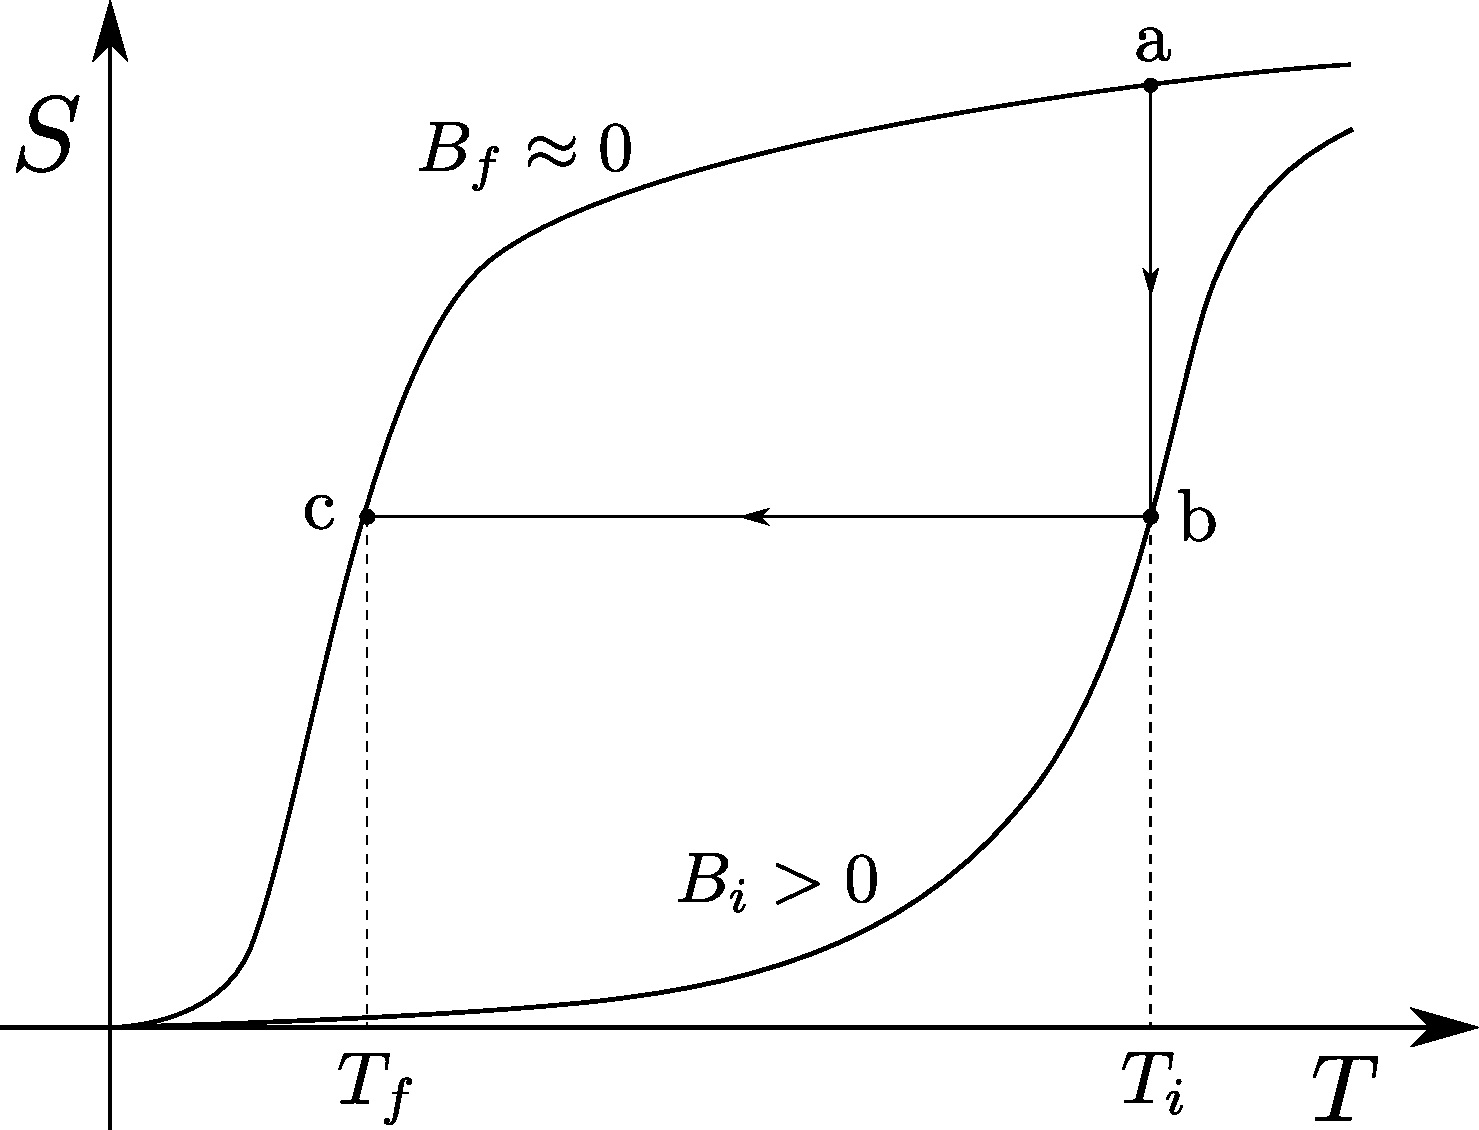
\includegraphics[width=\linewidth]{mag}
		\caption{سرمایش نمک پارامغناطیس به کمک یک فرایند هم‌دما و یک فرایند بی‌دررو}
		\label{fig1}
	\end{figure}
	به شکل \ref{fig1} دقت کنید. برای سرد کردن یک نمک پارامغناطیسی، ابتدا با استفاده از روش‌هایی مثل تبخیر هلیوم مایع آن را به دمای $T_i$ می‌رسانیم.
	با استفاده از هلیوم-4 می‌توانیم نمک را به دمای حدود 1 کلوین برسانیم و با استفاده از هلیوم-3 می‌توانیم دما را به 300 میلی کلوین کاهش دهیم.\footnote{
	علت بهینه‌تر بودن سرمایش توسط ایزوتوپ هلیوم-3 سبک‌تر بودن (یعنی کم‌تر بودن جرم) آن و عدم وجود پدیده ابرشارگی برای آن است؛
	سبک بودن به این کمک می‌کند که تبخیر سطحی راحت‌تر انجام بگیرد. پدیده ابرشارگی در هلیوم-4 باعث می‌شود بتواند روی تمام سطوح در دسترس پخش شود.
	با حرکت روی دیواره‌های ظرف و لوله‌های پمپ هلوم-4 به سمت نواحی گرم‌تر می‌رود و در آنجا بخار می‌شود که این عمل کارایی پمپ را پایین می‌آورد.
	همچنین مقداری از این بخار دوباره در نواحی سردتر چگالیده می‌شود و گرما آزاد می‌کند که بازدهی را پایین می‌آورد و دای تعادل سیستم را بالا می‌برد.}
	در این دما اثر گرما مغناطیسی مشهود است و می‌توانیم از آن برای سرد کردن نمک استفاده کنیم.
	در مرحله بعدی آنتروپی نمک را به صورت هم‌دما کم می‌کنیم (فرایند ab) و در آخر دمای آن را به صورت بی‌دررو پایین می‌آوریم (فرایند bc) تا به دمای $T_f$ برسیم.
	برای انجام فرایند همدما، نمک را با استفاده از یک محیط تبادلی در تماس با یک منبع هلیوم مایع قرار می‌دهیم و
	به آرامی میدان مغناطیسی بیرونی را قوی می‌کنیم تا به آنتروپی مطلوب برسیم (تبادل گرمای بین نمک و هلیوم مایع باعث می‌شود که دمای نمک ثابت بماند).
	سپس برای انجام فرایند بی‌دررو، نمک را از نظر گرمایی عایق می‌کنیم و میدان مغناطیسی بیرونی را به آرامی ضعیف می‌کنیم تا میدان کاملاً از بین برود
	(کند بودن این فرایند مهم است؛ باید زمان کافی برای تعادل بین دوقطبی‌های مغناطیسی با شبکه بلوری نمک و بقیه اجزایی که سرد می‌کنیم، وجود داشته باشد).
	بدین ترتیب می‌توانیم دمای نمک پارامقناطیس را تا حدود دمای کوری آن پایین ببریم؛ در این دما برهم‌کنش دوقطبی‌های مغناطیسی قوی است
	و جهت‌گیری خود به خودی اتفاق می‌افتد. این موضوع باعث می‌شود ماده به یک آهنربای دائمی تبدیل شود و اثر گرمامغناطیسی از بین برود.
	دمای کوری چند نمک پارامغناطیس مناسب برای سرمایش مغناطیسی در جدول \ref{tab} مشخص شده است. این فرایند سرمایش،
	\emph{مغناطیس‌زدایی بی‌دررو}\LTRfootnote{Adiabatic Demagnetization} نام دارد.
	\begin{table}
	\begin{center}
	\begin{LTR}
	\begin{tabular}{|c|O{c}|O{c}|O{c}|}
		\hline
		نوع & نام & ترکیب & \rl{دمای کوری ($T_c$)} \\ \hline
		\multirow{2}{*}{\rl{دما بالا}} & MAS & $\mathrm{Mn^{2+}SO_4\cdot(NH_4)_2SO_4\cdot6H_2O}$ & $\SI{0.17}{\kelvin}$ \\ \cline{2-4}
		& FAA & $\mathrm{Fe_2^{3+}(SO_4)_3\cdot(NH_4)_2SO_4\cdot24H_2O}$ & $\SI{0.03}{\kelvin}$ \\ \hline
		\multirow{2}{*}{\rl{دما پایین}} & CPA & $\mathrm{Cr_2^{3+}(SO_4)_3\cdot K_2SO_4\cdot24H_2O}$ & $\SI{0.01}{\kelvin}$ \\ \cline{2-4}
		& CMN & $\mathrm{2Ce^{3+}(NO_3)_3\cdot3Mg(NO_3)_2\cdot24H_2O}$ & $\SI{0.002}{\kelvin}$ \\ \hline
	\end{tabular}
	\end{LTR}
	\caption{مشخصات چند نمک پارامغناطیس مناسب برای سرمایش مغناطیسی\cite{pobell2007matter}}
	\label{tab}
	\end{center}
	\end{table}
	برای اینکه دمای کوری نمک پارامغناطیسی پایین باشد، می‌توانیم از نمک‌هایی استفاده کنیم که در شبکه بلور آنها فاصله دوقطبی‌های مغناطیسی نسبتاً زیاد است
	تا برهم‌کنش بین دوقطبی‌ها ضعیف باشد و جهت‌گیری خودبه‌خودی سخت‌تر اتفاق بیفتد. البته باید این را هم در نظر بگیریم که با کم شدن چگالی دوقطبی‌های مغناطیسی،
	سهم آنتروپی مغناطیسی (حاصل از به‌هم‌ریختگی جهت‌های دوقطبی‌های مغناطیسی) از آنتروپی کل کم می‌شود و توان سرمایشی نمک پارامغناطیسی کاهش می‌یابد.
	این موضوع هنگامی که از نمک برای سرد کردن نمونه دیگری (جز خود نمک) استفاده می‌کنیم، بسیار حائز اهمیت است.
	در کل باید بین دمای کمینه و توان سرمایشی تعادل مطلوبی ایجاد کنیم.
	
	می‌توانیم با استفاده از روابط مربوط به خواص مغناطیسی مواد و کمی محاسبه ریاضیاتی،
	رابطه‌ای بین مقادیر میدان مغناطیسی و دماها در فرایند بی‌دررو (مغناطیس‌زدایی بی‌دررو) بدست آوریم. طبق تعریف ظرفیت گرمایی در میدان مغناطیسی ثابت:
	\begin{equation}
		\pdvc{C_B}{B}{T} = \pdv{B}\qty(T\pdvc{S}{T}{B})_T = T\pdv{S}{B}{T}
	\end{equation}
	طبق تقارن مشتق جزئی مرتبه دوم:
	\begin{equation}
		\pdvc{C_B}{B}{T} = T\pdv{S}{T}{B} = T\pdv{T}\qty(\pdvc{S}{B}{T})_B
	\end{equation}
	طبق رابطه ماکسول \eqref{max}:
	\begin{equation}
		\pdvc{C_B}{B}{T} = T\pdv{T}\qty(\pdvc{M}{T}{B})_B = T\qty(\pdv[2]{M}{T})_B
	\end{equation}
	با جایگذاری از رابطه \eqref{der}:
	\begin{equation}
		\pdvc{C_B}{B}{T} = \frac{T B}{\mu_0}\qty(\pdv[2]{\chi_m}{T})_B
	\end{equation}
	وابستگی پذیرفتاری مغناطیسی به دما در دماهایی که خیلی به دمای کوری نزدیک نباشند از قانون کوری-وایس بدست می‌آید:
	\begin{equation}
		\chi_m = \frac{C}{T-T_c}
	\end{equation}
	که در آن $T_c$ دمای کوری و $C$ ثابتی وابسته به خواص ماده مغناطیسی است. با استفاده از این قانون:
	\begin{equation}
		\pdvc{C_B}{B}{T} = \frac{T B}{\mu_0}\qty[\frac{2C}{(T-T_c)^3}]
	\end{equation}
	حال از دو طرف معادله روی $B$ انتگرال می‌گیریم:
	\begin{align}
		\int_0^B \pdvc{C_B}{B}{T}\mathop{dB} &= \int_0^B \frac{2 C T B}{\mu_0(T-T_c)^3}\mathop{dB} \\
		\eval{C_B}_0^B &= \eval{\frac{C T B^2}{\mu_0(T-T_c)^3}}_0^B  \\
		C_B(B, T) &= C_B(0, T) + \frac{C T B^2}{\mu_0(T-T_c)^3}
	\end{align}
	جمله دوم مربوط به تغییر نظم حاصل از جهت‌گیری دوقطبی‌ها در میدان مغناطیسی است. جمله اول مربوط به بقیه عواملی است که در آنتروپی سیستم سهیم هستند.
	بخشی از آن مربوط به جنبش ذرات شبکه‌ای است که یون‌های مغناطیسی را دربر دارد و همچنین جنبش ذرات نمونه دیگری که توسط نمک درحال سرد شدن است.
	این سهم‌ها در دما‌های پایینی که سرمایش مغناطیسی در آن اتفاق می‌افتد، معمولاً ناچیز و قابل صرف‌نظر هستند.
	عامل دیگر مربوط به جمله اول، برهم‌کنش دوقطبی‌های مغناطیسی و جهت‌گیری خود به خودی در دمای نزدیک به دمای کوری است.
	می‌توانیم برای دما‌هایی که خیلی به دمای کوری نمک نزدیک نیستند، از این سهم نیز نیز صرف‌نظر کنیم. پس در بازه دمایی اصلی سرمای مغناطیسی با تقریب خوبی:
	\begin{equation}
		C_B(B, T) = \frac{C T B^2}{\mu_0(T-T_c)^3}
	\end{equation}
	با جایگذاری عبارت بالا در رابطه \eqref{adia2} و استفاده از قانون کوری-وایس:
	\begin{equation}
		\pdvc{T}{B}{S} = \frac{T-T_c}{B}
	\end{equation}
	با انتگرال گیری:
	\begin{equation} \label{magfin}
		\frac{T_f-T_c}{T_i-T_c} = \frac{B_f}{B_i}
	\end{equation}
	به عبارتی دیگر، نسبت میدان مغناطیسی اعمال شده و اختلاف دمای نمک پارامغناطیس تا دمای کوری آن، در فرایند بی‌دررو ثابت است.
	یعنی آنتروپی نمک پارامغناطیس تابعی از این نسبت است.
	
	با توجه به رابطه \eqref{magfin} با صفر شدن میدان مغناطیسی خارجی، دمای نمک پارامغناطیسی تا دمای کوری آن پایین می‌رود.
	در عمل، دما تا این حد کاهش نمی‌یابد چون در این تقریب، جهت‌گیری خودبه‌خودی دوقطبی‌های مغناطیسی را درنظر نگرفتیم که در نزدیکی دمای کوری
	تأثیر چشمگیری دارد و قابل صرف‌نظر نیست. پس دمای نهایی از دمای کوری کمی بالاتر خواهد بود.
	
	همچنین دقت کنید که میدان مغناطیسی اولیه‌ای که به سیستم اعمال می‌کنیم باید به اندازه کافی بزرگ باشد تا آنتروپی سیستم به حدی پایین بیاید که
	آنتروپی مغناطیسی با آنتروپی حاصل از جنبش ذرات و بقیه اثرات گرمایی، قابل مقایسه باشد.
	فقط در این صورت اثر مغناطیس‌زدایی بی‌دررو به اندازه‌ای بزرگ است که می‌تواند جنبش ذرات را تا حد قابل توجهی کاهش دهد و دما را پایین بیاورد.
	\section{یخچال رقیق‌سازی هلیوم-3/هلیوم-4}
	مرجع: \cite{pobell2007matter}
	
	\begin{figure}
	\centering
	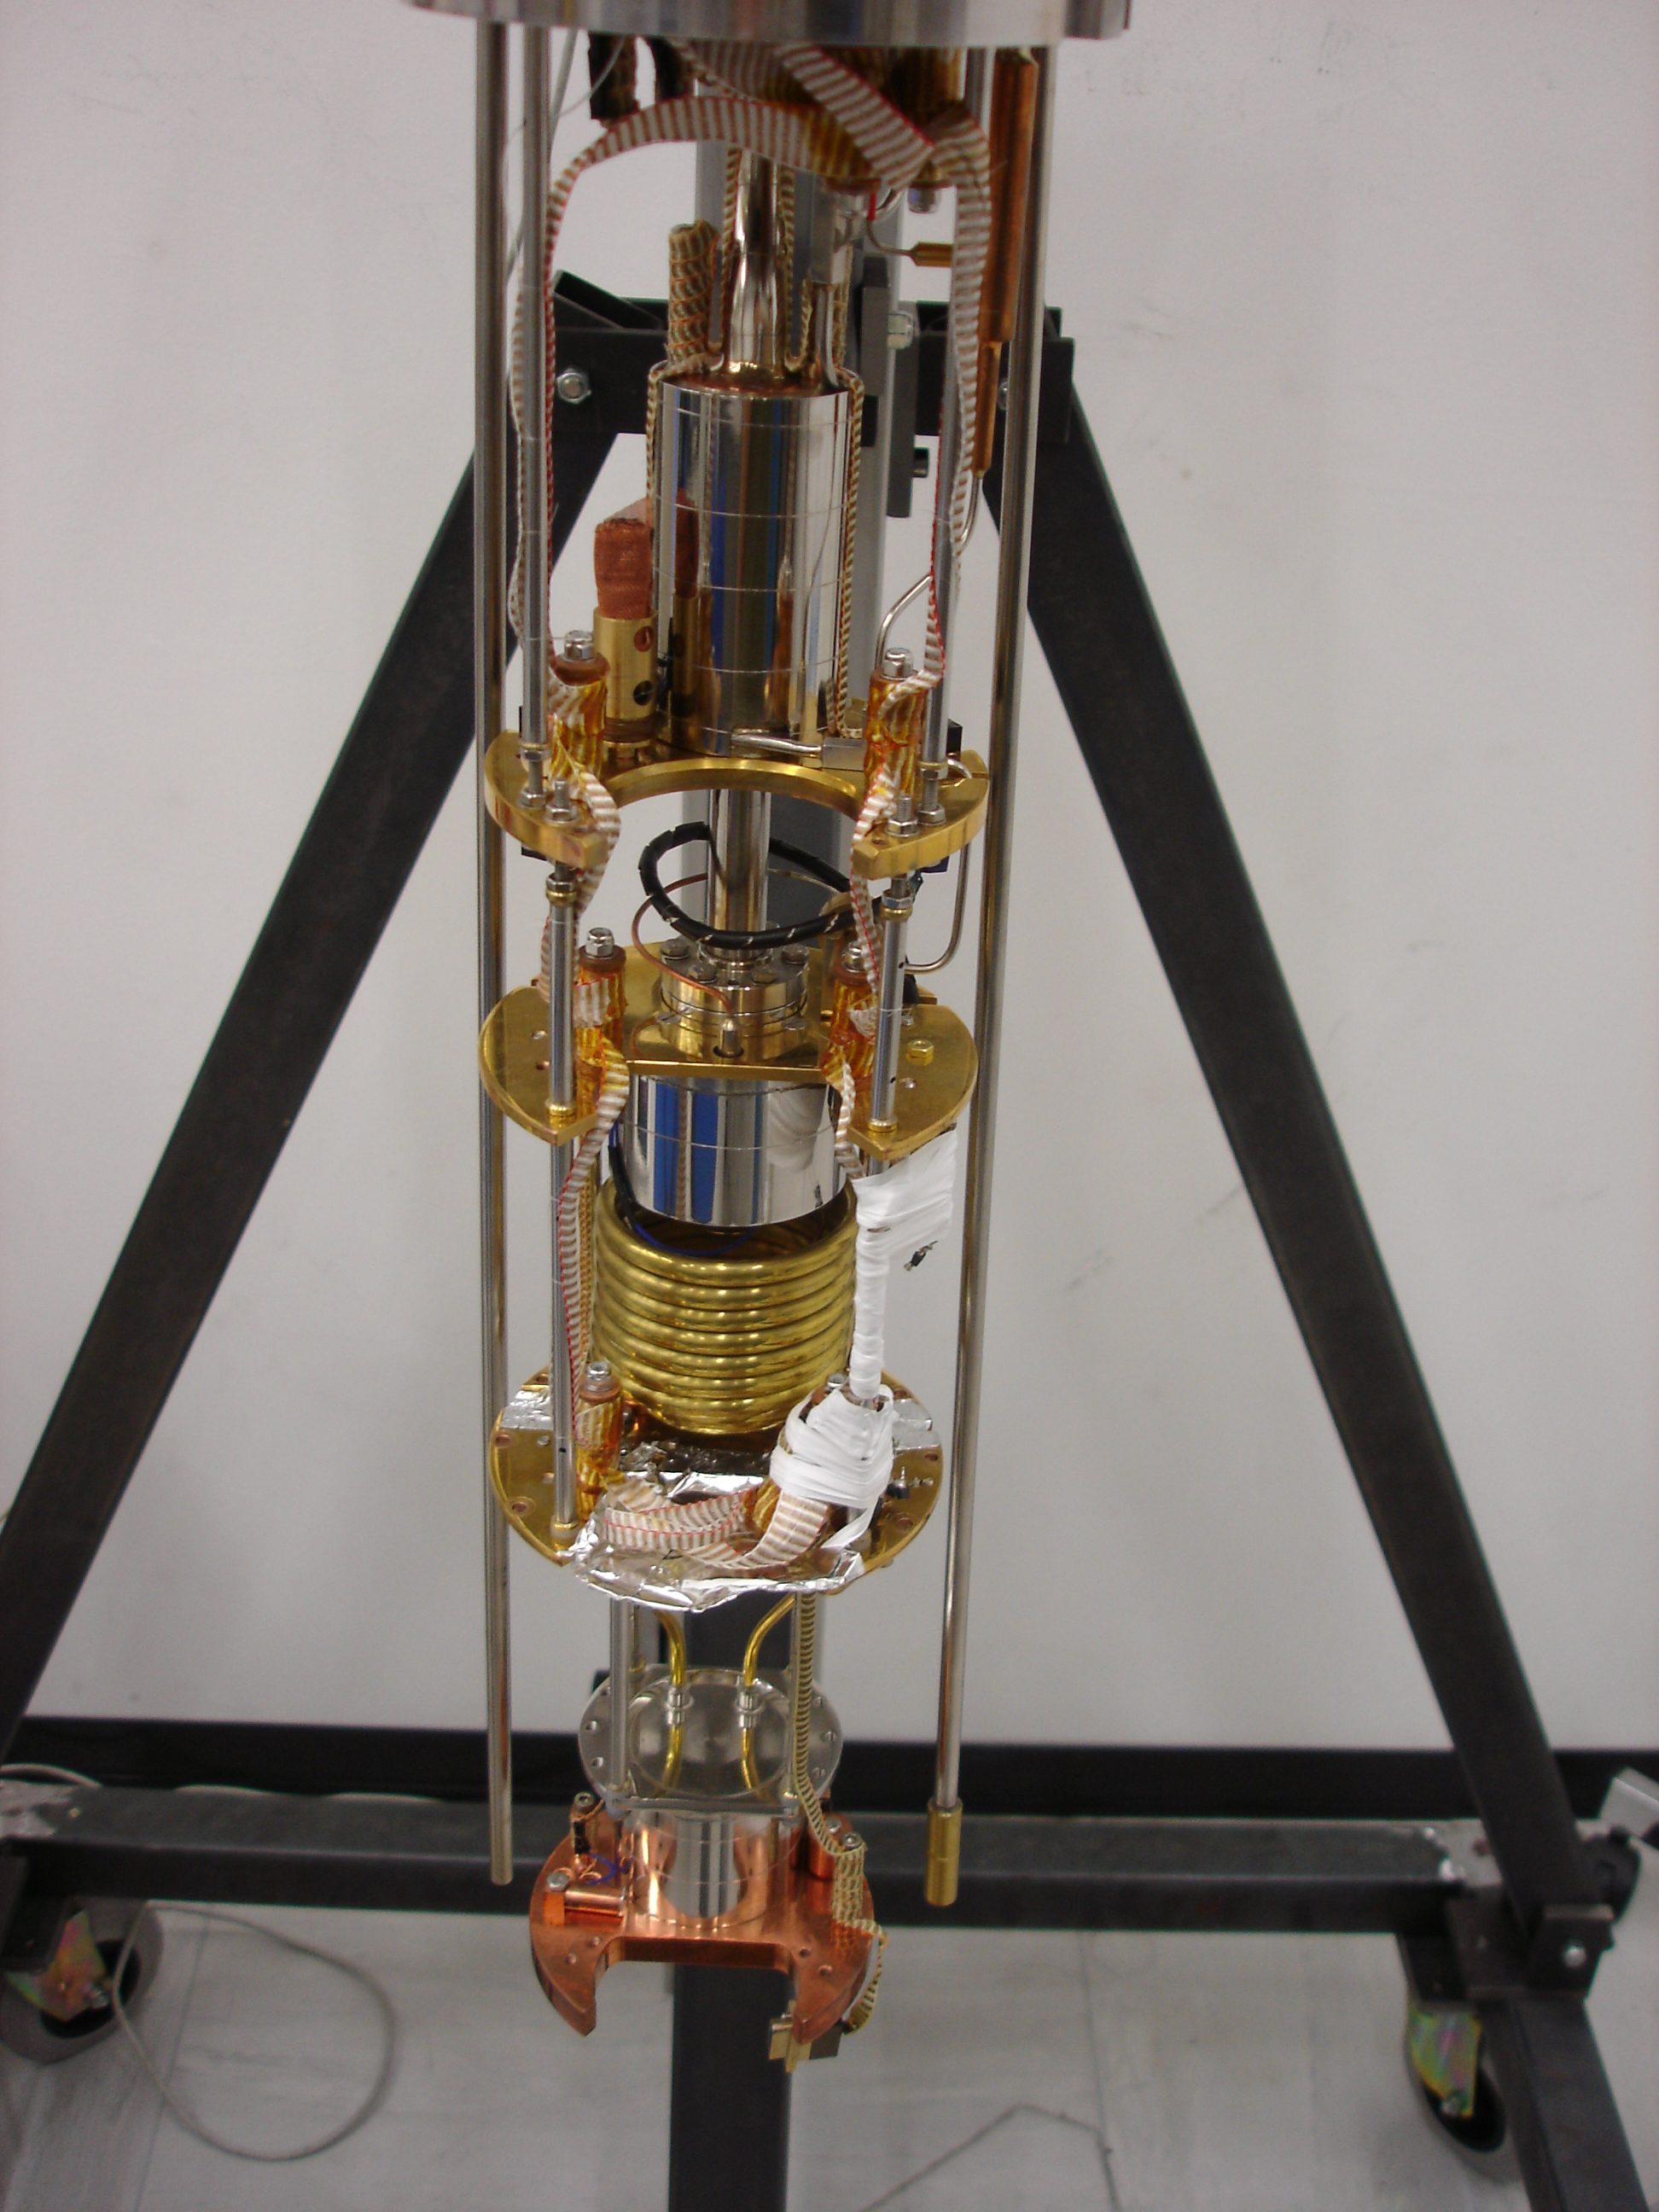
\includegraphics[width=\linewidth]{hdc}
	\caption{داخل یک یخچال رقیق‌سازی هلیوم \lr{Oxford Instruments}}
	\label{fig2}
	\end{figure}
	این روش از گرمای اختلاط محلول هلیوم-3 و هلیوم-4 برای سرمایش استفاده می‌کند.
	امرزوه این روش برای سرمایش در بازه دمایی 0.2 میلی کلوین تا 1 کلوین استفاده می‌شود.
	یخچال رقیق‌سازی هلیوم به نسبت پیچیدگی کمی دارد و ساختن آن در آزمایشگاه‌ها کار خیلی سختی نیست.
	یخچال‌هایی از این نوع برای سرمایش تا دمای $\SI{4}{\milli\kelvin}$ در بازار وجود دارد.
	
	تا حدود دهه 1950 تنها روش دستیابی دماهای پایین یک کلوین، سرمایش مغناطیسی بود. این روش در بازه 0.3 تا 1 کلوین با سرمایش تبخیری هلیوم-3 جایگزین شد.
	در سال 1962 روش سرمایش جدیدی توسط هاینتز لاندن\LTRfootnote{Heinz London}، ج. ر. کلارک\LTRfootnote{G. R. Clarke} و ای. مندوزا\LTRfootnote{E. Mendoza}
	پیشنهاد داده شد (ایده اولیه آن ده سال قبل از آن توسط لاندن ارائه داده شده بود) که در آن به جای تبخیر، از اختلاط هلیوم-3 و هلیوم-4 مایع استفاده استفاده می‌شود.
	در سال 1965 برای اولین بار این ایده توسط تیمی از دانشگها لایدن\LTRfootnote{Leiden University} عملی شد.
	این تیم با یخچال رقیق‌سازی خود به دمای $\SI{0.22}{\kelvin}$ دست یافتند. یک سال بعد، تیمی از دوبنا\LTRfootnote{Dubna}
	با استفاده از همین روش به دمای $\SI{25}{\milli\kelvin}$ دست یافتند.
	\subsection{جدایی فاز مخلوط و انحلال پذیری}
	\begin{figure}
		\centering
		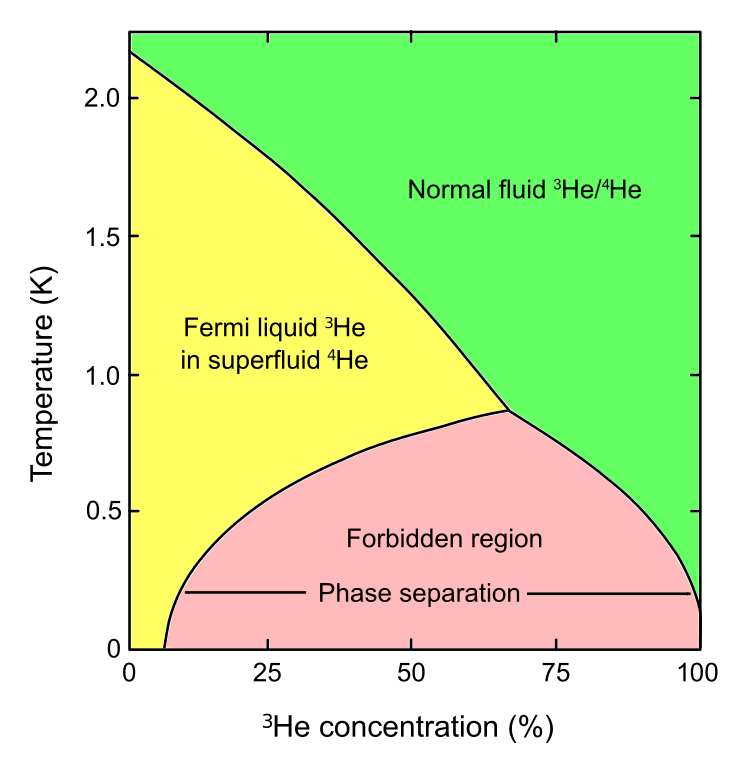
\includegraphics[width=0.75\linewidth]{phase}
		\caption{نمودار فاز مخلوط هلیوم-3/هلیوم-4 که جدایی فازها را نشان می‌دهد}
		\label{fig3}
	\end{figure}
	اساس کار یخچال رقیق‌سازی هلیوم، جدایی فاز مخلوط هلیوم-3/هلیوم-4 است. به شکل \ref{fig3} دقت کنید؛ هلیوم-4، که از آمار بوز-اینشتین تبعیت می‌کند،
	در دمای $\SI{2.177}{\kelvin}$ به ابرشاره تبدیل می‌شود اما هلیوم-3، که از آمار فرمی-دیراک پیروی می‌کند، در بازه دمایی کار یخچال رقیق‌سازی هیچ گذار فازی به ابرشارگی ندارد.
	دمای گذار فاز به ابرشارگی در مخلوط هلیوم-3/هلیوم-4 با افزایش غلظت هلیوم-3 پایین می‌رود و در غلظت $67.5\%$ این ایزوتوپ، دیگر فاز ابرشارگی برای مخلوط وجود ندارد.
	در این غلظت و در دمای $\SI{0.867}{\kelvin}$ خط $\lambda$ خط جدایی فاز را قطع می‌کند. پایین‌تر از این دما دو ایزوتوپ هلیوم فقط غلظت‌های خاصی با هم مخلوط می‌شوند.
	اگر دمای یک محلول هلیوم را از $\SI{0.867}{\kelvin}$  کم‌تر کنیم، محلول جدا می‌شود و دو فاز غلیظ و رقیق (نسبت به هلیوم-3) تشکیل می‌دهد.
	با پایین آمدن دما، محلولی که هلیوم-3 بیشتری دارد (محلول غلیظ)، غلیظ‌تر می‌شود و در حالت حدی دمای صفر مطلق، این بخش حاوی هلیوم-3 خالص خواهد بود.
	اما چنین رفتاری در محلولی که هلیوم-4 بیشتری دارد (محلول رقیق) دیده نمی‌شود و در حالت حدی دمای صفر مطلق، غلظت هلیوم-3 مقدار ثابت $6.6\%$ خواهد بود.
	اگر $x_3 $ و $x_4 $ به ترتیب غلظت هلیوم-3 در محلول رقیق و غلظت هلیوم-4 در محلول غلیظ باشند، در دماهای پایین و فشار بخار اشباع:
	\begin{empheq}[left=\empheqlbrace]{align}
		x_4 &= 0.85 T^{3/2}e^{-0.56/T} \\
		x_3 &= 0.066(1+8.3T^2), \quad T < 0.1K
	\end{empheq}
	در دمای صفر مطلق، بیشینه انحلال‌پذیری هلیوم-3 در هلیوم-4، $9.5\%$ در فشار $\SI{10}{\bar}$ است. کمینه انحلال‌پذیری آن $6.6\%$ در فشار صفر است.
	
	در دمای نزدیک صفر مطلق، هلیوم-3 فضای بیشتری از هلیوم-4 اشغال می‌کند چون سبک‌تر است (این باعث می‌شود انرژی نقطه صفر آن بالاتر باشد).
	پس نیروی جاذبه بین یک اتم هلیوم-3 و یک اتم هلیوم-4 قوی‌تر از نیروی جاذبه بین دو اتم هلیوم-3 است.
	به همین دلیل حالتی که در آن تعدادی از اتم‌های هلیوم-3 در بین اتم‌های هلیوم-4 قرار بگیرند، از حالتی که اتم‌های دو ایزوتوپ کامل از هم جدا باشند پایدارتر است.
	از طرفی نیروی جاذبه بین دو اتم هلیوم-4 از نیروی جازبه بین یک اتم هلیوم-3 و یک اتم هلیوم-4 قوی‌تر است. این عامل و برهم‌کنش‌های مغناطیسی بین اتم‌های هلیوم-3
	میان اتم‌های هلیوم-4 و آمار فرمی-دیراک، باعث می‌شوند پایدارترین حالت برای سیستم، حالتی باشد که در آن تعداد کمی از اتم‌های هلیوم-3 میان اتم‌های هلیوم-4 قرار بگیرند.
	این تحلیل‌ها برای بازه دمایی صادق است که در آن آمار فرمی-دیراک و اثرات کوانتومی غالب می‌شوند.این دما در واقع همان دمایی است که در آن جدایی فاز شروع می‌شود.
	در دما‌های بالاتر، مکانیک آماری کلاسیک (آمار مکسول-بولتزمن) غالب است و هلیوم-3 و هلیوم-4 می‌توانند آزادانه با هم مخلوط شوند.
	\subsection{ساز و کار سرمایش}
	\begin{figure}
		\centering
		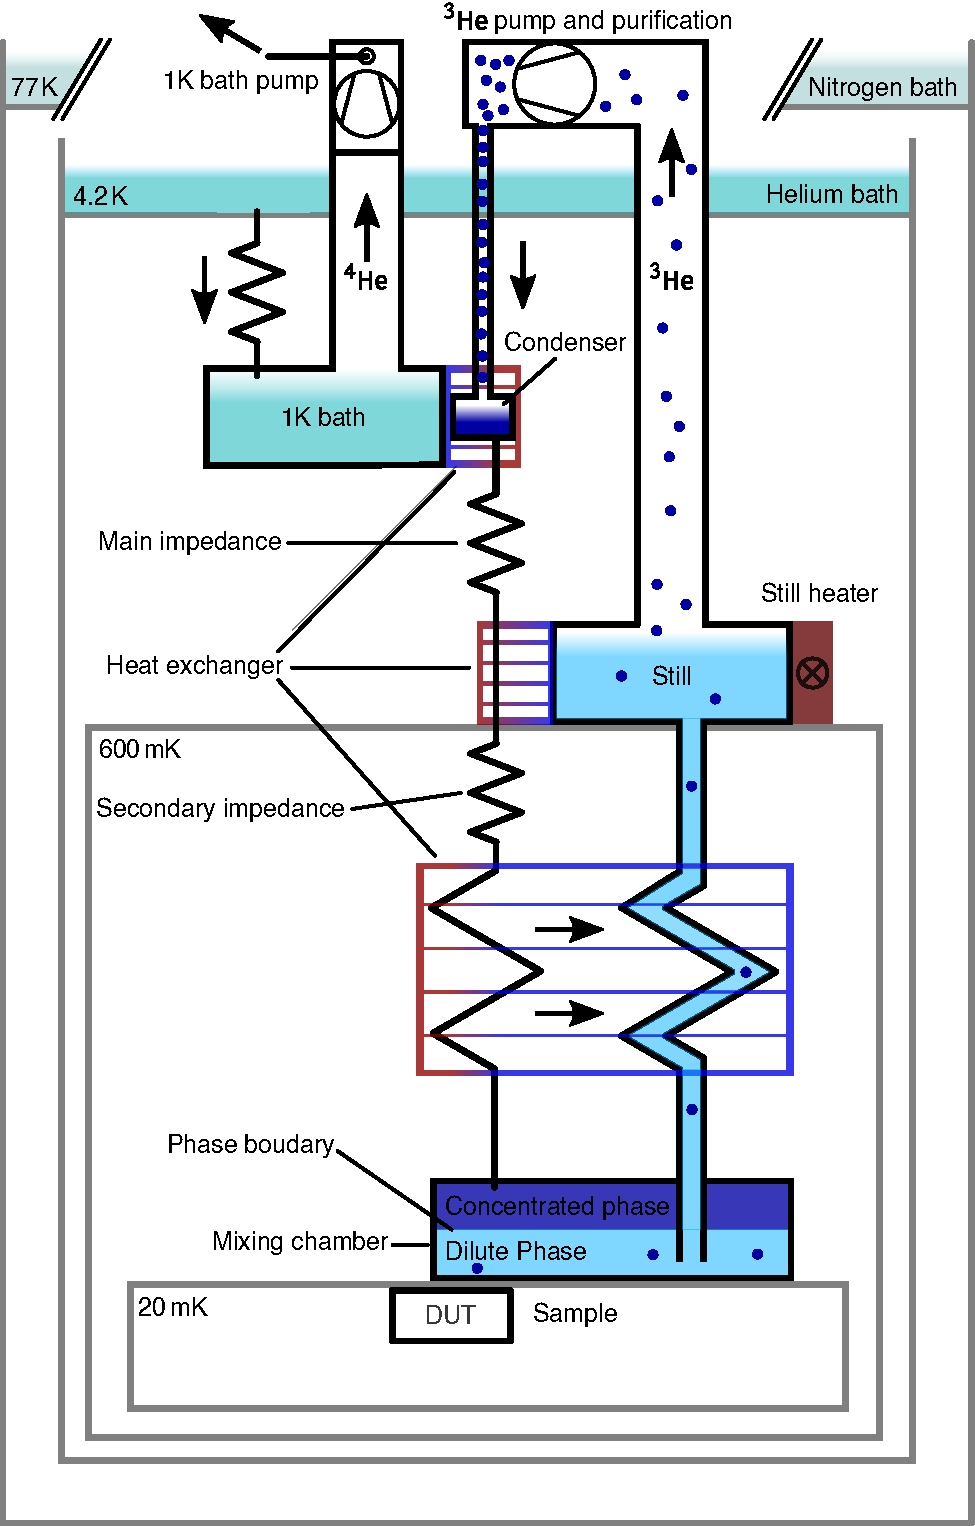
\includegraphics[width=0.9\linewidth]{cooler}
		\caption{شکل شماتیک یخچال رقیق‌سازی هلیوم}
		\label{fig4}
	\end{figure}
	در یخچال رقیق‌سازی هلیوم، عامل سرمایش نفوذ هلیوم-3 داخل محلول رقیق است؛ هنگام مخلوط شدن دو ماده، آنتروپی سیستم بالا می‌رود چون بی‌نظمی افزایش پیدا می‌کند.
	پس با مخلوط شدن دو فاز محلول هلیوم از طریق نفوذ هلیوم-3 از محلول غلیظ به رقیق، گرما جذب می‌شود و از این طریق می‌توانیم از یک نمونه گرما بگیریم و آن را سرد کنیم.
	
	به شکل \ref{fig4} دقت کنید. در \emph{مخزن اختلاط}\LTRfootnote{Mixing Chamber} یخچال که در مجاورت نمونه‌ای است که می‌خواهیم سرد کنیم،
	مخلوط هلیوم در دو فاز رقیق و غلیظ نسبت به هلیوم-3 موجود است و محلول‌های این دو فاز در تماس با یکدیگر قرار دارند.
	محلول رقیق توسط لوله‌ای به بخش \emph{تقطیرگر}\LTRfootnote{Still} یخچال وصل است. تقطیرگر در دمایی کمی بالاتر از نقطه جوش هلیوم-3 قرار دارد.
	چون هلیوم-3 از هلیوم-4 سبک‌تر است و نیروی بین ذره‌ای در آن کمی ضعیف‌تر است، نقطه جوش آن از هلیوم-4 پایین‌تر است.
	این باعث می‌شود با گرما دادن به محلول تقطیرگر، هلیوم-3 خیلی بیشتر از هلیوم-4 تبخیر شود (گرما صرف تبخیر می‌شود و دما ثابت می‌ماند).
	پس غلظت هلیوم-3 داخل تقطیرگر کم می‌شود که فشار اسمزی از مخزن اختلاط به سمت تقطیرگر ایجاد می‌کند.
	بدین ترتیب، هلیوم-3 در مخزن اختلاط با فشار اسمزی داخل محلول غلیظ کشیده می‌شود و با نفوذ آن و مخلوط شدن، آنتروپی بالا می‌رود و گرما از نمونه بیرونی جذب می‌شود.
	بخار هلیوم-3 از تقطیرگر پمپ می‌شود و از طریق میعان، به مخزن اختلاط باز گردانده می‌شود. این گونه چرخه سرمایشی کامل می‌شود.
	\subsection{توان سرمایشی}
	به دلیل آنتروپی اختلاط، آنتالپی هلیوم-3 در حالتی که در محلول رقیق قرار دارد، بیشتر از حالتی است که در محلول غلیظ قرار دارد.
	پس توان سرمایش از رابطه زیر بدست می‌آید (فشار در طول فرایند نفوذ، تقریبا ثابت است):
	\begin{equation} \label{power}
		\dot{Q}=\dot{n}_3[h_d(T) - h_c(T)]
	\end{equation}
	در رابطه بالا $\dot{n}_3 $ تعداد مول‌های هلیوم-3 است که در واحد زمان از محلول غلیظ به محلول رقیق نفوذ پیدا می‌کند
	و $h_c(T)$ و $h_d(T)$ به ترتیب آنتالپی هر مول هلیوم-3 در محلول غلیظ و رقیق در دمای $T$ است. با صرف نظر از تأثیرات مربوط به فشار و حجم:
	\begin{equation}
		h(T) - h(0) = \int_0^T c(T)\mathop{dT}
	\end{equation}
	که در آن $c(T)$ ظرفیت گرمایی ویژه در دمای $T$ است. برای محلول غلیظ هلیوم-3، تئوری خوبی برای بررسی آماری آن وجود ندارد. طبق اندازه‌گیری‌های تجربی:
	\begin{equation}
		c_c(T)=22T \quad [\si{\joule\per\mole\per\kelvin}]
	\end{equation}
	با انتگرال گیری:
	\begin{equation} \label{h_c}
		h_c = h(0) + 11T^2 \quad [\si{\joule\per\mole}]
	\end{equation}
	برای محلول رقیق، می‌توانیم هلیوم-3 داخل آن را یک گاز فرمی در نظر بگیریم چون غلظت آن کم است. بنابراین:
	\begin{equation}
		c_d(T) = R\frac{\pi^2}{2}\frac{T}{T_F}
	\end{equation}
	که $T_F$ دمای فرمی است که از رابطه زیر بدست می‌آید:
	\begin{equation}
		T_F = \frac{\hbar^2}{2m*k_B}\qty(\frac{3\pi^2 N_A x_3}{V_m})^{2/3} = 55.2\frac{m_3}{m*}\qty(\frac{x}{V_m})^{2/3}
	\end{equation}
	($N_A$ عدد آووگادرو و $m*$ جرم مؤثر است) حجم مولی $V_m$ از رابطه زیر بدست می‌آید:
	\begin{equation}
		V_m = V_{m, 4}(1+0.284x_3)
	\end{equation}
	که در آن $V_{m, 4} = \SI{27.589}{\centi\meter\cubed\per\mole} $ حجم مولی هلیوم-4 مایع خالص است. با قرار دادن $x_3=0.066 $ و $m* \approx 2.5m_3 $،
	دمای فرمی $T_F$ حدوداً برابر $\SI{0.38}{\kelvin}$ بدست می‌آید و:
	\begin{equation}
		c_d(T) = 106 T \quad [\si{\joule\per\mole\per\kelvin}]
	\end{equation}
	چون دو محلول در تعادل ترمودینامیکی قرار دارند، پتانسیل شیمیایی آنها برابر است:
	\begin{equation}
		\mu_c = \mu_d
	\end{equation}
	طبق رابطه اویلر برای انرژی درونی و رابطه آنتالپی با انرژی درونی:
	\begin{equation}
		h = u + pv = Ts + \mu
	\end{equation}
	پس طبق برابری پتانسیل‌های شیمیایی:
	\begin{equation}
		h_c - Ts_c = h_d + Ts_d
	\end{equation}
	طبق تعریف ظرفیت گرمایی ویژه $c = \dbar Q_m/dT = T(ds/dT)$ و رابطه \eqref{hc}:
	\begin{align}
		h_d &= h_c(0) + 11T^2 + T\int_0^T \qty(\frac{c_d}{T} - \frac{c_c}{T})\mathop{dT} \\
		&= h_c(0) + 95T^2 \quad [\si{\joule\per\mole}]
	\end{align}
	با جایگذاری در رابطه \eqref{power}، توان سرماشی یخچال رقیق سازی هلیوم بدست می‌آید:
	\begin{equation}
		\dot{Q}(T) = \dot{n}_3T^2
	\end{equation}
	طبق داده‌های تجربی، $\dot{n}_3 \approx \SI{100}{\micro\mole\per\second}$ و:
	\begin{empheq}[left=\empheqlbrace]{align}
		\dot{Q}(\SI{10}{\milli\kelvin}) &\approx \SI{1}{\micro\watt} \\
		\dot{Q}(\SI{30}{\milli\kelvin}) &\approx \SI{10}{\micro\watt}
	\end{empheq}
	وابستگی درجه دو توان سرمایشی از دما، باعث می‌شود یخچال رقیق‌سازی در دما‌های زیر یک کلوین از سرمایش تبخیری بسیار مؤثرتر واقع شود؛ چراکه برای سرمایش تبخیری:
	\begin{equation}
		Q \propto e^{-1/T}
	\end{equation}
	و به همین دلیل توان سرمایش تبخیری در دماهای پایین، بسیار کمتر از توان سرمایشی یخچال رقیق‌سازی است چون با کم شدن دما، با سرعت بیشتری (به طور نمایی) به صفر میل می‌کند.
	\setLTRbibitems
	\bibliographystyle{plain}
	\bibliography{ref}
	\section*{منابع شکل‌ها}
	شکل \ref{fig1} را به طور کیفی خودم کشیدم \\ \\
	شکل \ref{fig2}: \\
	\lr{\parbox{\linewidth}{\url{https://en.wikipedia.org/wiki/File:Helium_dilution_cryostat.jpg}}} \\ \\
	شکل \ref{fig3}: \\
	\lr{\parbox{\linewidth}{\url{https://en.wikipedia.org/wiki/File:Helium_phase_diagram.svg}}} \\ \\
	شکل \ref{fig4}: \\
	\lr{\parbox{\linewidth}{\url{https://en.wikipedia.org/wiki/File:Sketch_of_helium_dilution_refrigerator.svg}}}
\end{document}